\documentclass[11pt,leqno,oneside]{amsart}

\usepackage{../notes}
\newcommand{\Arg}{\operatorname{Arg}}
\newcommand{\Log}{\operatorname{Log}}
\newcommand{\Res}{\operatorname{Res}}
\renewcommand{\Re}{\operatorname{Re}}
\renewcommand{\Im}{\operatorname{Im}}
%%%%%%%%%%%%%% BEGIN CONTENT: %%%%%%%%%%%%%%

\title[Complex Analysis]{Complex Analysis}
\author{George H. Seelinger (inspired from class by David Sherman)}
\date{Fall 2016}
\begin{document}
\maketitle
\section{Lecture 1}
What makes complex analysis different than calculus and real analysis?

\begin{enumerate}
    \item Over the complex field, all polynomials factor completely.
    \item All the functions are infinitely differentiable and can thus be written as a power series.
    \item It is easier to describe important physics problems using complex analysis to solve partial differential equations.
    \item Some integrals can be solved using visual tricks and some integrals that are not solvable using calculus/real analysis omit solutions using complex analysis.

\end{enumerate}
\begin{example}
    The polynomial $x^2+10x+100$ cannot be factored in terms of real factors since its discriminant is negative. However, this can be factored over the complexes.
\end{example}
\begin{example}
    Describing physical phenemenon, such as the flow of a river over a log, is much easier using complex analysis.
\end{example}
\begin{example}
    Solving $\int_{-\infty}^{\infty} \frac{\cos 2x}{x^2+1} dx$ is almost impossible for a standard calculus student and in real analysis, one can show that the integral is finite, but solving it is difficult. In complex analysis, one can easily show that it is $\pi^2/e$.
\end{example}
\begin{example}
    $\int_{\gamma} \frac{\cos z}{z} dz = 2 \pi i $ times the number of counter clockwise rotations around $(0,0)$ in the complex plane.
\end{example}
\section{Lecture 2}
When doing complex analysis, it is important to develop a geometric intuition
for what is happening when you see functions of complex variables. The
following are some examples:
\begin{table}
    \centering
    \begin{tabular}{|c|c|}
        \hline
        $|z-w|$ & The distance from $z$ to $w$ \\
        $|z-1|=|z-i|$ & The locus of points equidistance from $1$ and $i$, ie a line. \\
        $|z-1|=3-|z-i|$ & The distance from $z$ to 1 and $z$ to $i$ add to 3, ie a parabola. \\
        $|z-1|=3+|z-i|$ & The upper part of a hyperbola (because the complex ordering). \\
        $|z-1|=2|z-i|$ & A circle (points that are twice as far from $1$ as from $i$). \\
        $|z-1|=\frac{2}{|z-i|}$ & An oval shape called a Cassini oval (product of distances is constant). \\
        \hline
    \end{tabular}
    \caption{Some real functions in complex form}
    \label{tab:func-descs}
\end{table}
Also note that $\ov{z}$ is $z$ reflected over the x-axis.

In $\R$, there are many ways to define $e^x$. One way is $e^x =
\sum_{n=0}^\infty \frac{x^n}{n!}$. We can define $\sin$, $\cos$, and other functions in complex $x$ using taylor series expansions.
\[
    e^{ix} = 1 + ix + \frac{(ix)^2}{2!} + \frac{(ix)^3}{3!} + \cdots = \cos x + i \sin x
\]
By splitting $e^{ix}$ into its real and imaginary parts, we obtain power series for $\sin(x)$ and $\cos(x)$.
\begin{align*}
  e^{ix} =& \sum_{n=0}^\infty \frac{(ix)^n}{n!}  \\
  =& \sum_{n\ \text{even}}^\infty \frac{(ix)^n}{n!} + \sum_{n\ \text{odd}}^\infty \frac{(ix)^n}{n!} \\
  =& \sum_{n\ \text{even}}^\infty \frac{i^n x^n}{n!} + i\sum_{n\ \text{odd}}^\infty \frac{i^{n-1} x^n}{n!} \\
  =& \cos(x) + i \sin(x)
\end{align*}

When $x$ is real, $|e^{ix}| = |\cos x + i \sin x| = \sqrt{\cos^2 x + \sin^2 x}
= 1$, so our rules in $\R$ still hold.

This formulation allows us to come up with the polar form of looking at complex
numbers. This boils down to $z = r e^{i \theta}$ where $r = |z|$ and $\theta
\in \arg z$. Note that $\arg z$ is the \emph{set} of (real) $\theta$ that solve
the equation. However, since $\arg$ is multi-valued, we say that $\Arg \in
\arg$ is the value that is between $(-\pi, \pi]$.

From this description, we get that $e^z e^w = e^{z+w}$ (follows from the power series). In particular, $(e^z)^n = e^{nz}, n \in \N$, This gives us \[
    \cos n \theta + i \sin n \theta = e^{in\theta} = (e^{i\theta})^n = (\cos \theta + i \sin \theta)^n
\]
This formula is often called \emph{DeMoivre's formula} and from it, we can
recover trig identities by expanding and equating the real and imaginary parts.

Overall, polar form is good for understanding multiplication and powers. For example, $\frac{1}{z} = \frac{1}{r} \exp{-i \theta}$.

We can also take roots effectively using polar form (look it up).

Finally, we can look at the stereographic projection (see textbook for picture) using the one-point compactification of $\C$, namely $\C^* = \C \cup \{\infty\} \cong S^2$.

We also get some nice correspondances from actions on the sphere as in the table. \\
    \begin{tabular}{|c|c|}
        \hline
        Equator & $|z| = 1$ \\
        Upper hemisphere & $\{|z| > 1\} \cup \{\infty\}$ \\
        Lines of lattitude & Circle centered at origin \\
        Lines of longitude & Rays from origin \\
        Circles on $S^2$ that do not contain the north pole & Circles on $\C^*$ \\
        Circles on $S^2$ that contain the north pole & Lines on $\C^*$ \\
        \hline
    \end{tabular}
\section{Lecture 3}

Let us continue to understand some basic functions in on $\C$. \\
\begin{tabular}{|c|c|}
    \hline
    $f(z) = iz$ & Rotation counter-clockwise by $\frac{\pi}{2}$. \\
    $f(z) = (1+i)z$ & Rotation counter-clockwise by $\frac{\pi}{4}$ and dilation by $\sqrt{2}$. \\
    $f(z) = z^2$ & Squares modulus and doubles the argument. \\
   \hline
\end{tabular} \\
Let us also examine $f(z) = z^{\frac{1}{2}} = \{w | w^2=z\}$. This is a multivalued function satisfying
\begin{align*}
    (|w|e^{i\theta})^2 = |z|e^{i \arg z} & \implies \begin{cases}
        |w|^2 = |z| \implies |w| = \sqrt{|z|} \\
        2\theta \in \arg z \implies \theta = \frac{\Arg z}{2}, \frac{\Arg z + 2\pi}{2}
    \end{cases} \\
    \ & \ \implies \ w = \sqrt{|z|}e^{\frac{\Arg z}{2}i}, \sqrt{|z|}e^{\frac{\Arg z + 2\pi}{2} i}
\end{align*}
\begin{defn}
    A \emph{domain} is an open subset of $\C$ where every pair of points can be connected by a broken line segment.
\end{defn}
\begin{defn}
    A branch of a multivalued function is a (continuous) choice of output on some domain.
\end{defn}
\begin{example}
    $z \mapsto \sqrt{|z|}e^{\frac{\Arg z}{2}i}$ is the principal branch of
    $z^{\frac{1}{2}}$ on $\C \smallsetminus (-\infty,0]$.
\end{example}

Now, let us consider $f(z) = e^z$. This is $f(z) = e^{x+iy} = e^x(\cos y +
i\sin y)$. Notice that $e^x$ is the modulus and $\cos y + i \sin y$ is the
argument. We also note that $e^z$ maps a grid of cartesian coordinates into a
grid of polar coordinates.

Next, consider the inverse of $e^z$, namely $\log z$ on $\C \smallsetminus
\{0\}$. We get that $\log z = w \implies e^w = z = e^{\Re w} \cdot e^{i \Im w}
= |z|e^{i \arg z}$. Thus we get that $\Re w = \ln|z|$ and $\Im w \in \arg z$.
When we take $\Im w = \Arg z$, we get $\Log z$. It is instructive to look at a
picture of $\Log z$'s graph.

From the above, we also note that $\cos z = \frac{e^{iz}+e^{-iz}}{2}$ and $\sin
z = \frac{e^{iz}-e^{-iz}}{2i}$. These identities are also useful for finding
$\cos^{-1}$ and $\sin^{-1}$. Also note that $\cosh z = \frac{e^z+e^{-z}}{2}$
and $\sinh z = \frac{e^z-e^{-z}}{2}$. In this sense, $\cosh$ and $\sinh$ are
rotations of $\cos$ and $\sin$ in the complex plane.

Coming back to the function $z^{\frac{1}{2}}$, it is important to discuss the
branch cut of the function. This creates a 1 dimensional complex manifold or
2 dimensional real manifold (plus some structure). A good treatement of this
will not be found here, but refer to any standard complex analysis textbook.

\section{Lecture 4}
When considering the stereographic projection representation of the complex
plane, consider that the following actions on the sphere have the following
effects in $z$.

\begin{tabular}{|c|c|}
    \hline
    Reflection over $xy$ & $f(z) = \frac{1}{\overline{z}}$ \\
    Reflection over $yz$ & $f(z) = -\overline{z}$ \\
    Reflection over $xz$ & $f(z) = \overline{z}$ \\
    Rotation by $\pi$ around $x$ & $f(z) = \frac{1}{z}$ \\
    Rotation by $\pi$ around $y$ & $f(z) = \frac{-1}{z}$ \\
    Rotation by $\pi$ around $z$ & $f(z) = -z$ \\
    \hline
\end{tabular}

To get a group out of these actions, one needs to add $f(z) = z$ and $f(z) =
\frac{-1}{\overline{z}}$. This forms a certain group of isometries on the
surface of a sphere ($\cong \Z_2 \times \Z_2 \times \Z_2$). This means that
these maps will map circles on a sphere to other circles on a sphere, which
also means that circles and lines on a complex plane will be mapped ot circles
and lines on a complex plane.

Actually note that the group $O(3)$ (of 3 by 3 matrices) is the group of all
isometries of the sphere. Geometrically, there are 4 types of isometries
\begin{enumerate}
    \item The identity
    \item Reflection over a plane
    \item Rotation around an axis
    \item A glide reflection (rotation then reflection over the equator).
\end{enumerate}
Note, just items 1 and 3 form the group $SO(3)$.

\begin{defn}
    Functions of $z$ that are orientation perserving are known as conformal
    maps and are also analytic. Similarly, functions of $\overline{z}$ are
    orientation flipping and are thus anti-conformal maps and are also
    anti-analytic.
\end{defn}

Treatment of phase factors is skipped because it is difficult to write up
without pictures.

\section*{Analysis Review}

\begin{defn}
A domain in $\C$ is convex if, for any two points in the domain, the line
between them is also contained in the domain.
\end{defn}
\begin{defn}
    A domain in $\C$ is star-shaped if there exists a point for which, when a
    line is drawn between it and any other point in the domain, the line is in
    the domain. Note that all convex domains are star-shaped, but not the other
    way around.
\end{defn}
\begin{defn}
    Let $f: \C \to \C$ be defined on a domain containing $z$. If $\lim_{\Delta
    z \to 0} \frac{f(z+\Delta z) - f(z)}{\Delta z}$ exists in $\C$, this number
    is called the \emph{derivative of $f$} at $z$ and we say that $f$ is
    differentiable at $z$.
\end{defn}

``Usual examples'' include $f(z) = z^n \implies f'(z) = nz^{n-1}$. Also note
that $f(z) = \overline{z}$ is not differentiable anywhere because the value of
the limit changes depending on if you approach in the real direction or the
imaginary direction.
\begin{defn}
    $f$ is \emph{analytic} on a domain if it is differentiable at all points on
    the domain and $f'(z)$ is continuous.
\end{defn}
We will see that the second assumption is superflous when we prove Goursat's
theorem later.

\begin{thm}
    Let $f(x+iy) = u(x,y)+iv(x,y)$ be defined on a domain. Then it is analytic
    if and only if $u,v$ satisfy the Cauchy-Riemann equations $u_x = v_y, u_y =
    -v_x$ and these partials are continuous.
\end{thm}
\begin{proof}
    Assume $f$ is analytic. Then, take the limits of $\Delta z$ along the
    imaginary axis and the real axis and then equate. This should yield the
    Cauchy-Riemann equations.

    Conversely, take the Cauchy-Riemann equations and show that the limit
    exists using Cauchy-Riemann equations.
\end{proof}
\section{(9/6/2016) Lecture 5: Landau Notation and Cauchy-Riemann Equations}
\begin{rmk*}
    An aside at the beginning of lecture: recall $|z+i||z-i|=c$ from homework.
    It is true that any equation of the form $|p(z)| = c$ where $p$ is a
    complex polynomial and $c$ a nonnegative constant forms curves called ovals
    of Cassini. These are generally called polynomial lemniscetes. An open
    Erdos conjecture is as follows: \\

    All monic polynomials of degree $n$, the length of the polynomial
    lemniscete $|p(z)|=1$ is maximized by $z^n-1$.
\end{rmk*}

    A second aside about confusion concerning branch points and branch cuts.
    The general situation is that we have a multivalued function and we want to
    define a branch of it on some domain. Some things that could happen at 0:
    \\
    \begin{tabular}{|c|c|}
        \hline
        $\frac{1}{z}$ & Singly valued on $\C \smallsetminus \{0\}$, 0 is not a
        branch point. \\
        $z^{\frac{1}{2}}$ & Defined on 0, but 0 is a branch point. This yields
        a phase factor of $-1$. \\
        $\log z$ & 0 is a branch point, but there is no phase factor. \\ \ & Instead
        you add $2\pi i$ on a counter-clockwise loop. \\
        \hline
    \end{tabular}
    Recall that a branch point is a point where the one cannot define a
    continuous branch in a deleted neighborhood of the point. The minimum
    situation for all these listed functions with 0 as a branch point is that
    one can remove path from 0 to $-\infty$ from the domain.

    To emphasize further, ``the branch of $z^\frac{1}{2}$ on $\Re z > 1$ that
    is negative at 2'' is a valid sentence.

    \subsection*{Landau (``big oh'') notation}
    The idea behind Landau notation is that we want to bound one function in
    terms of another as the input $x$ goes to some $c$ (typically either 0 or
    $\infty$). This idea is used a lot in computer science and is an integral
    part of complexity analysis.

    \begin{defn}
        Say that $f$ is $O(g)$ if there is a positive $M$ in a neighborhood of
        $c$ where $|f(x)| \leq M|g(x)|$.
    \end{defn}
    Note, if there is a neighborhood where $g \neq 0$, this say that
    $\frac{|f(x)|}{|g(x)|}$ is bounded near $c$.
    \begin{defn}
        $f$ is $o(g)$ if $\forall \epsilon > 0$, there is a neighborhood of $c$
        where $|f(x)| < \epsilon |g(x)|$.
    \end{defn}
    Here, if there is a neighborhood where $g \neq 0$, this says that
    $\frac{|f(x)|}{|g(x)|} \to 0$.\\

    It is important to note that language here gets abused frequently.

    \begin{example}
        (At $\infty$), $f$ is $O(x^6)$, $g$ is $O(x^4)$. Then, $f+g$ is
        $O(x^6)$ and $fg$ is $O(x^{10})$.
    \end{example}

    Some further consequences are that $f$ is bounded is the same as saying $f$
    is $O(1)$ and that saying $f$ goes to 0 is the same as saying $f$ is
    $o(1)$.

    \subsection*{Returning to differentiation}

    \begin{defn}
        A restatement of differentiability is that $f$ is differentiable at $x$
        if and only if $\exists c$ such that $f(x+\Delta x) = f(x) + c \Delta x
        + o(\Delta x)$ and if $f$ is differentiable, $c$ is the derivative of
        $f$ at $x$. Note that the $o(c)$ captures the essential notion of the
        derivative, since it essentially states that the error must go to zero
        and must be $o(\Delta x)$, ie, the error must approach zero faster than
        $\Delta x$.
    \end{defn}
    Note that the statement for complex differentiability is the same, but
    replace all $\Delta x$ by $\Delta z$ and replace $o(\Delta x)$ with $o(|
    \Delta z|)$. Now for an application: prove the Leibniz rule (product rule
    of differentiation) using landau notation.
    \begin{proof}
        \begin{align*}
            f(x+\Delta x)g(x+\Delta x) & = (f(x)+f'(x)\Delta x + o(\Delta
            x))(g(x)+g'(x) \Delta x + o(\Delta x)) \\
            \ & = f(x)g(x) + \Delta x(f'(x)g(x)+g'(x)f(x)) \\
            \ & \ + f'(x)f'(x)(\Delta
            x)^2 + f'(x)(\Delta x)o(\Delta x) + \dots \\
            & = f(x)g(x) + \Delta x(f'(x)g(x) + g'(x)f(x)) + o(\Delta x)
        \end{align*}
        Note the abusive notation, but it gets the desired result since the
        $o(\Delta x)$ terms go to 0 and thus the derivative is
        $f'(x)g(x)+g'(x)f(x)$.
    \end{proof}

    Now, recall that we had a theorem stating that a function is analytic if
    and only if it satisfies the Cauchy-Reimann equation.
    \begin{proof}
        Let us examine $f'(z) = \lim_{\Delta z \to 0} \frac{f(z+\Delta z) -
        f(z)}{\Delta z}$. Taking $\Delta z = \Delta x$ real, then $f'(z) =
        \lim_{\Delta x \to 0} \frac{u(x+\Delta x, y)+iv(x+\Delta x,y) -
        (u(x,y)+iv(x,y))}{\Delta x} = u_x(x,y)+iv_x(x,y)$.

        Similarly, taking $\Delta z = i \Delta y$, we get $f'(z) = \frac{u(x,
        y+ \Delta y) + iv(x+,y+\Delta y)}{i\Delta y} = -iu_y+v_y$. Thus,
        setting both parts equal, we get $v_x = -u_y$ and $u_x = v_y$.

        We will now prove the converse using Landau notation instead of limits.
        Now, we know that $f(z+\Delta z) =
        u(x + \Delta x, y + \Delta y) + iv(x+\Delta x, y + \Delta y)$. We will
        choose to work with the real part first.
        \begin{align*}
            u(x+\Delta x, y + \Delta y)  & = u(x, y+ \Delta y) + \Delta x
            u_x(x,y+\Delta y) + o(\Delta x) \\
            \ & \text{ using the }x\text{ derivative.} \\
            \ & = u(x,y) + \Delta y u_y(x,y) + o(\Delta y) + \Delta x
            u_x(x,y+\Delta y) + o(\Delta x) \\
            \ & \text{ using the }y\text{ derivative.} \\
            \ & = u(x,y) + \Delta y u_y(x,y) + o(\Delta y) + \Delta x
            (u_x(x,y)+o(1)) + o(\Delta x) \\
            \ & \text{ using the continuity of }u_x\\
            \ & = u + \Delta y u_y + \Delta x u_x + o(\Delta y) + o(1)\Delta x
            + o(\Delta x) \\
            \ & = u + \Delta y u_y + \Delta x u_x + o(|\Delta z|)
        \end{align*}
        Similarly, we can do this to get $iv(x+\Delta x, y + \Delta y) =
        i(v+\Delta y v_y + \Delta x v_x + o(|\Delta z|))$. So now, continuing
        with $f$ and applying the Cauchy-Riemann equations, we get
        \begin{align*}
            f(z+\Delta z) & = u + iv + \Delta y (-v_x) + \Delta x u_x + i\Delta
            y u_x + i \Delta x v_x + o(|\Delta z|) \\
            \ & = u + iv + \Delta z(u_x+iv_x)+o(|\Delta z|)
        \end{align*}
        So, $f'(z) = u_x+iv_x$, which we assumed continuous, so $f$ is analytic.
    \end{proof}
    \section{(9/8/2016) Lecture 6: Developing Intuition for Complex Differentiation}
    In class, we first completed an exercise imagining the graph of $2i$
    raised to various powers. The end result was that these graphs always
    produce (possibly degenerate) spirals. Two graphs are provided here,
    but once raised to a complex power, the graphs produce spirals that
    increase their modulus exponentially, and so, at scale, the graph is rather
    unenlightening.

    \begin{figure}[h]
        \centering
        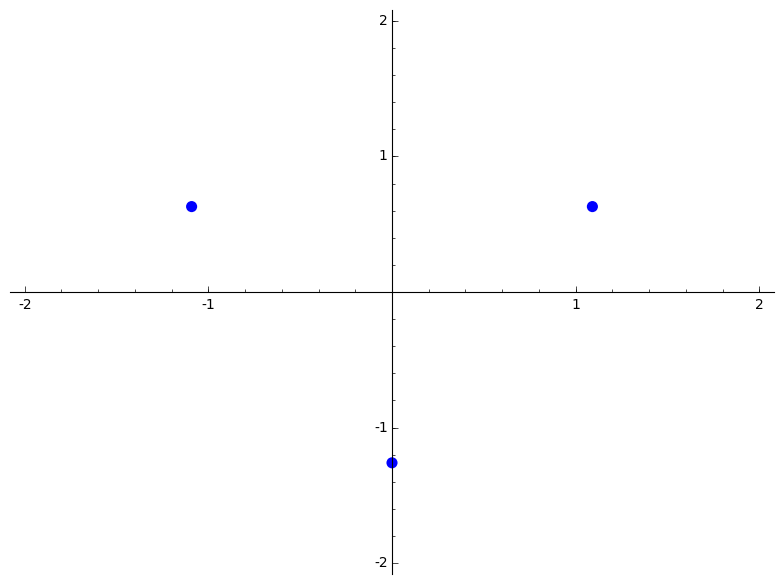
\includegraphics[scale=0.2]{images/2i-to-one-third.png}
        \caption{$2i^{\frac{1}{3}}$}
        \label{fig:2i13}
    \end{figure}
    \begin{figure}[h]
        \centering
        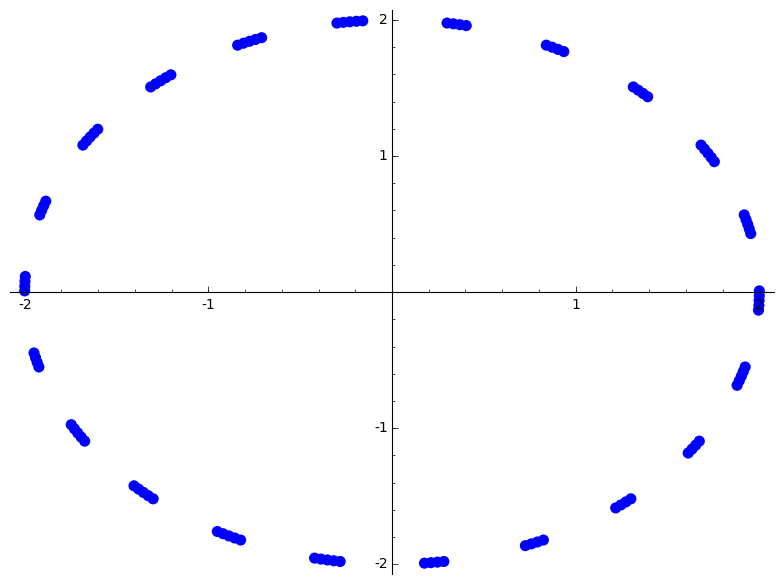
\includegraphics[scale=0.2]{images/2i-to-1-over-pi.png}
        \caption{$2i^{\frac{1}{\pi}}$ first $k = 0,1, \ldots, 100$}
        \label{fig:2i1pi}
    \end{figure}

    Now, a general definition of differentiability for $\R^n$ spaces is as
    follows.
    \begin{defn}
        A function $f: \R^m \to \R^n$ is differentiable at $x$ if $f(x+h) =
        f(x)+D(h)+o(h)$ where $D: \R^m \to \R^n$ is linear (a matrix). In fact,
        $D$ is the Jacobian matrix of partial derivatives and $f(x)+D(h)$ is
        the tangent plane.
    \end{defn}
    For a complex function $f: \C \to \C$, we write $f = u+iv$ where $u,v: \R^2
    \to \R$. When $u,v \in C^1$, $D = \left( \begin{array}{cc}
        u_x & u_y \\
        v_x & v_y
    \end{array}\right)$. As a reminder, complex differentiability happens when
    we have real differentiability plus the function satisfied the
    Cauchy-Riemann equations. Then, note that $\det D = u_x^2 + v_x^2 =
    |u_x+iv_x|^2 = |f'(z)|^2$. Thus a function $z+h \mapsto f(z) + f'(z)h$
    dilates $h$ by $|f'(z)|$ and rotates it by $\arg f'(z)$. The consequence of
    this is that analytic maps take squares in the input to squares in the
    output and they are orientation preserving. Thus, we get the following
    \begin{rmk}
        If $f$ is analytic on $D$, $z \in D, f'(z) = 0$, then there is a
        neighborhood $U$ with $z \in U \subset D$ on which $f$ is one-to-one
        with analytic inverse satisfying $(f^{-1})'(f(z)) = \frac{1}{f'(z)}$.
        This is the inverse function theorem and it applies since the Jacobian
        is invertible.
    \end{rmk}
    A natural question to then ask is how are branches affected by
    differentiation. Let us show a few examples.
    \begin{example}
        \begin{enumerate}
            \item $\frac{d}{dz}(\log z) = \frac{1}{z}$ where we are using any
                branch of $\log$. $z = e^{\log z} \implies 1 = e^{\log z} \cdot
                (\log z)' \implies \frac{1}{z} = (\log z)'$. Thus, the choice
                of branch for $\log$ does not affect the derivative in this
                case.
            \item $\frac{d}{dz}(z^{\frac{1}{2}})$ depends on the branch. $z =
                (z^{\frac{1}{2}})^2 \implies 1 =
                2(z^{\frac{1}{2}}(z^{\frac{1}{2}})'$ which gives us
                $(z^{\frac{1}{2}})' = \frac{1}{2(z^\frac{1}{2})}$. Thus, the
                $z^\frac{1}{2}$ in the final result is the same branch as the
                branch that was differentiated.
        \end{enumerate}
    \end{example}

    \begin{defn}
        A function $u: \R^n \to \R$ is \emph{harmonic} if it is a $C^2$
        solution to $\Delta u = 0$. Note that $\nabla^2u = \Delta u$ and is
        called the Laplacian.
    \end{defn}
    Harmonic functions will turn out to be $C^\infty$, but we cannot prove this
    yet. Note also that if $f = u+iv$ is analytic, then $u$ is harmonic. This
    follows because $u_{xx}+u_{yy} = u_{xx}+(-v_x)_y = u_{xx}-v_{yx} =
    u_{xx}-u_{xx} = 0$. There is an almost converse which states that ``a
    harmonic function is locally the real part of an analytic function.'' That
    is, on a neighborhood of any point, there is a $v$ with $u+iv$ analytic locally.
    Such a $v$ is called a \emph{harmonic conjugate} (unique up to an additive
    constant), e.g., there is an $x$ such that $u=xy$ satisfying \[
        \begin{cases}
 u_x = v_y = y \\
 u_y = -v_x = x. \\
    \end{cases}
\]
This is a PDE satisfied by the solution $\frac{y^2-x^2}{2} + C$. So, we get
that $xy+i\left( \frac{y^2-x^2}{2} \right)$ is analytic. In terms of $z$, this
conjugate is $f(x) = \frac{-iz^2}{2}$. Also note that the local part of the
definition is necessary. For instance $\frac{1}{2} \log(x^2+y^2)$ is harmonic
on $\R^2 \smallsetminus \{(0,0)\}$. \\

Some follow up facts to note are
\begin{itemize}
    \item All harmonic functions of $\R$ have the form $ax+b$.
    \item $u+v$ is harmonic.
    \item $uv$ is not harmonic.
    \item $u_x$ is harmonic.
    \item If $v$ is a harmonic conjugate of $u$, the harmonic conjugate of $v$
       is $-u$. Thus, note that harmonic conjugation is not an unordered pair.
    \item $u+iv$ is analytic implies that $v-iu$ is analytic.
\end{itemize}
\subsection*{Conformal Maps}
\begin{defn}
    If $f$ is analytic in a neighborhood at $z_0$ and $f'(z_0) \neq 0$, then
    $f$ is \emph{conformal} at $z_0$. This is the same as saying directed
    angles are preserved by $f$ at $z_0$.
\end{defn}
\begin{defn}
    A \emph{conformal mapping} between domains is a one-to-one $C^1$ function
    that is conformal at each point.
\end{defn}
Note the following implications.
\begin{itemize}
    \item $f: D \to V$ that is one-to-one and analytic is conformal.
    \item If $f$ is analytic at $z_0$ and $f'(z_0) \neq 0$, then $f$ maps a
        neighborhood of $z_0$ conformally onto the image.
\end{itemize}

\section{(9/13/2016) Lecture 7}
In general, a real differentiable function from $\R^2 \to \R^2$ will map some
small square to some small parallelogram modulo a small
perturbation. Furthermore, the ratio of the areas is the determinant of the
Jacobian. Now, if $f: \C \to \C$ is analytic and if $f'(z) \neq 0$, the map will
map a small square to another square modulo a small amount of error. This is an
essential difference between these types of functions. Thus, analytic maps are
conformal where $f' \neq 0$. \\

What if $f' = 0$?
\begin{example}
  Take $f(z) = z^2$ at 0. Then, $f(z)$ doubles angles, and is thus not angle
  preserving and thus not conformal at 0.
\end{example}

\begin{defn}
  A \emph{conformal equivalence} between domains is a one to one onto
  conformal/analytic map between them.
\end{defn}
\begin{example}
  $\{-\frac{\pi}{2} < \Im z < \frac{\pi}{2}\}$ is conformall equivalent to
  $\{\Re z > 0\}$ using the map $f(z) = e^z$.
\end{example}

A general question in complex analysis is ``given two domains, find a conformal
equivalence if one exists.''

Since conformal maps preserve angles, it is key to note they preserve
orthogonality.

\begin{rmk}
  Harmonic functions are exactly the functions that are locally the real parts
  of analytic functions. That is, given $u$, there exists on a neighborhood of
  any point and a $v$ defined on that neighborhood such that $u+iv$ is
  analytic.
\end{rmk}

\begin{example}
  \textbf{Non-example}: $\ln r$ on $\R^2 \smallsetminus \{(0,0)\}$. There is no
  harmonic conjugate that works for the entire domain. A harmonic conjugate
  would be a branch of $\arg$, so $z \mapsto \ln|z|+i\arg z$ would have to be
  analytic. However, that is not possible since no branch of $\arg$ can be
  continuous for the entire domain.
\end{example}

\subsection{Linear Fractional Transformations}
\begin{defn}
    A \emph{linear transformation} is of the form $az + b$ with $a,b \in \C$.
\end{defn}
\begin{defn}
    An \emph{affine transformation} is a nonzero linear transformation.
\end{defn}
\begin{defn}
    A \emph{linear fractional transformation} is a map of the form $z \mapsto
    \frac{az+b}{cz+d}$ with $a,b,c,d \in \C$ and $ad-bc \neq 0$. These are also
    called fractional linear transformations and M{\"o}bius transformations.
  \end{defn}

  Some facts about LFTs:
  \begin{itemize}
  \item LFTs are unchanged if $a,b,c,d$ all multiplied by $\lambda \neq 0$.
  \item LFTs are defined at $\infty$.
  \item LFTs are one-to-one, onto maps from $\hat{\C} \to \hat{\C}$ with
    derivative non-zero. Thus, they are exactly the conformal equivalences from
    $\hat{\C} \to \hat{\C}$.
  \item LFTs are closed under inverse and composition. Thus, they have a group
    structure. A good treatment of this is in Gamelin in section II.7.
  \item Given distinct $z_1,z_2,z_3$ and distinct $w_1,w_2,w_3$, these exists a
    unique LFT taking $z_i$ to $w_i$.
    \item An LFT is a composition of linear maps and the inversion
      $\frac{1}{z}$. So, an LFT takes circles in $\hat{\C}$ to circles in
      $\hat{\C}$.
  \end{itemize}

  \subsection{Line Integrals}
  Line integrals are integrals of the form $\int_\gamma Pdx + Qdy$ where
  $\gamma$ is a path. To solve these, one usually parametrizes the path or uses
  theorems such as Green's theorem.
  \begin{defn}
    We call the integrand \emph{closed} if $P_y = Q_x$. We call the integrand
    \emph{exact} if there exists an $h(x,y)$ such that $h_x = P, h_y = Q$. Thus,
    if we have $h_xdx+h_ydy$, we would say this is an ``exact differential with
    $h$ as a primitive.''
  \end{defn}
  Note that if a vector field is exact, that is the same as saying it is
  independent of path or that integrals over loops are 0.
  \begin{rmk}
    \begin{itemize}
    \item If a differential is exact, then it is closed.
    \item If a differential is closed on a star-shaped domain, it is exact
    \end{itemize}
  \end{rmk}
  \begin{example}
    $\frac{-ydx+xdy}{x^2+y^2} = \Im \frac{1}{z}dz$ on $\R^2 \smallsetminus
    \{(0,0)\}$ is closed but not exact.
  \end{example}
  Finally, to make notions of path precise, we have the following.
\begin{defn}
    A \emph{path} is a continuous parametrized function $f:[a,b] \to \C$.  A
    path is \emph{simple} if it is injective (ignoring the endpoint).  A path is
    \emph{closed} if $f(a) = f(b)$.  The \emph{trace} of a path is its image
    $f([a,b])$.  A path is \emph{smooth} if $f(t)$ can be expressed as $(x(t),
    y(t))$ for $x$ and $y$ smooth (such a path is also called a \emph{curve}).
    A \emph{piecewise} path is a concatenation of paths (two paths must share an
    endpoint to be concatenated).
  \end{defn}

  Finally, we conclude with the following
  \begin{thm}
    A harmonic function on a star shaped domain has a harmonic conjugate.
  \end{thm}
  \begin{proof}
    Suppose $u$ is harmonic, then $-u_ydx+u_xdy$ is closed. So, it is also
    exact. Let $v$ be a primitive. Then $v_x = -u_y, v_y=u_x$. Thus, $u+iv$ is
    analytic. (Check this proof.)
  \end{proof}
  \section{(9/15/2016) Lecture 8}
  Integrals of closed forms $\{Pdx+Qdy, Q_x = P_y\}$ are invariant
  when
  \begin{itemize}
  \item the path is deformed, fixing endpoints.
  \item a loop is deformed.
  \end{itemize}

  A physical application would be with fluid flow. The example
  provided in class is a the top half of a log lying at the bottom of
  a riverbed. We can create a conformal equivalence with $f(z) =
  z+\frac{1}{z}$ between the flow lines of this river and the flow
  lines of a river with no log.

  \begin{defn}
    A function on $\R^2$ (or $\R^n$) has the \emph{mean-value
      property} (MVP) on a domain if its value at any point is the
    average of its values on any sufficiently small circle (or sphere)
    centered at the point. In other words, $u(z_0) = \frac{1}{2\pi}
    \int_0^{2\pi} u(z_0+re^{i\theta}) d\theta$.
  \end{defn}
  An amazing consequence of this definition is that it is the same
  thing as being harmonic. In Gamelin, there is a treatment about how
  harmonic on $\R^2$ implies MVP. The idea is that $\frac{d}{dr}$(
  average on circle of radius $r$) $=0$. Then, the average is
  continuous as $r \to 0$, so the averages must all be $u(z_0)$. \\

  Note that, in $\R$, MVP implies harmonic (linear).

  \subsection*{Maximum Principles}

  \begin{thm}[``Strict Maximum Principle'' for real harmonic functions]
    If $u$ is a harmonic, real-valued function and $u \leq M$ on a
    domain and $u(z_0) = M$ for some $z_0$, then $u \equiv M$. This is
    the same as saying ``no peaks or pits.''
  \end{thm}
  \begin{proof}
    By MVP, $u(z_0)$ is the average of its values at a sufficiently
    small circle centered at $z_0$, but these values are all $\leq M$,
    so they must all be $M$. So, $u \equiv M$ on a small disk centered
    at $z_0$. So $\{u = m\}$ is open. It is also open by continuity of
    $u$. A non-empty clopen subset of a domain is the whole domain, so
    $u \equiv M$.
  \end{proof}

  \begin{thm}[Strict maximum principle for complex harmonic functions]
    Same as above principle, except $|f(z)| \leq M$ and $|f(z_0)| =
    M$.
  \end{thm}
  \begin{proof}
    We may assume $M \neq 0$. Then $|f(z_0)| = M \implies f(z_0) =
    Me^{i\theta}$. Consider the same hypothesis holds for
    $e^{-i\theta}f$, so $u = \Re e^{-i\theta}f$. Then, $u \leq M$ and
    $u(z_0) = M$. So by previous theorem, $u \equiv M$, $M \geq
    |e^{-i\theta}f| \geq u \equiv M$. This tells us that
    $e^{-i\theta}f \equiv M \implies f = Me^{i\theta}$.
  \end{proof}
  \begin{thm}[``Maximum modulus principle'']
    If $f$ is complex harmonic on a bounded domain and extends
    continuously to the boundary, then $f$ attains its maximum modulus
    on the boundary.
  \end{thm}
  \begin{proof}
    $|f|$ is continuous on compact $D$, so the maximum is attained
    somwhere ?? in 0, so $f$ is constant by previous theorem. CHECK THIS!
  \end{proof}
  \section{(9/20/2016) Lecture 9: Complex Line Integrals}
  A complex line integral is an integral of the form $\int_\gamma
  f(z)dz$ where $\gamma$ is some path in the complex plane, $f(z)$ is
  some complex valued function, and $dz = dx + idy$. Just like a real
  integral, it can be phrased as $\lim \sum_{i=1}^n
  f(z_i^*)(z_{i+1}-z_i)$ and can be evaluated by parametrizing the
  path and function. \\

  We can also provide an upper bound on such integrals by noting the
  following:
  \begin{align*}
    |\int_\gamma f(z)dz | & \cong |\sum f(z)(z_{i+1}-z_i)| \\
    \ & \leq \sum |f(z_i^*)||s_{i+1}-z_i| \\
    \ & \leq \max_\gamma |f(z)| \sum |z_{i+1}-z_i| \\
    \ & \cong \max_\gamma |f(z)| \cdot \int_\gamma ds \\
    \ & (\max |f(z)|)(\operatorname{length} \gamma)
  \end{align*}
  This is called the ML estimate.

  \begin{example}
    Consider $\oint_{|z|=R} z^n dz$. We can parametrize this with
    $z(t) = Re^{it}, t \in (0,2\pi]$. Then, $z'(t) = iRe^{it}$ and we
    get our integral to be $\int_0^{2\pi} (Re^{it})^n iRe^{it} dt =
    R^{n+1} i \int_0^{2\pi} e^{it(n+1)} dt =
    \begin{cases}
      0 & \text{ if } n \neq -1 \\
      2 \pi i & \text{ if } n=-1
    \end{cases}.$
  \end{example}
  However, just like in calculus, we can also evaluate integrals using
  primitives or anti-derivatives. A primitive for $f$ is an analytic
  $F$ with $F'=f$.
  \begin{thm}[Fundamental Theorem of Calculus (Complex Version)]
    $\int_\gamma F'(z)dz = F(\text{end}) - F(\text{start})$
  \end{thm}
  This statement is exactly the same as the standard version.
  \begin{example}
    Consider $\oint_{|z|=R} z^n dz$. If $n \neq 1$, then $z^n$ has
    primitive $\frac{z^{n+1}}{n+1}$ on $\C \smallsetminus
    \{0\}$. However, if $n=-1$, primitives of $\frac{1}{z}$ are
    branches of $\log z$ and thus cannot be continuously defined on
    $|z|=R$.
  \end{example}
  In notes, there is a proof, but I am not sure why it is there...
  \begin{thm}
    If $f$ is analytic on a star-shaped (simply connected) domain,
    then it has a primitive.
  \end{thm}
  \begin{proof}
    Let $f=u_iv$. Consider $udz-vdy$. This differential is closed
    because $u_x = v_y$ by the Cauchy-Riemann equations. Now, since it
    is closed on a star-shaped domain, it is exact. So, there exists a
    $U$ with $U_x = u$ and $U_y = -v$ by definition of exact. Now,
    also note that $U$ is harmonic because $\Delta U = U_{xx} + U_{yy}
    = u_x-v_y = 0$ where the last equality follows from the
    Cauchy-Riemann equations. So, $U$ has a harmonic conjugate $V$
    since it is on a star-shaped domain. Thus, we have $F = U+iV$ that
    is analytic and note that $F' = U_x + iV_x = U_x-iU_y = u+iv = f$.
  \end{proof}
  Note that in this situation, we have $F(z) = \int_{z_0 \to z}
  f(z)dz$ is well-defined where $z_0 \to z$ is any path from $z_0$ to
  $z$.
  \section{(9/22/2016) Lecture 10: Integral Formulas}
  Continuing from above, we ask what happens if the domain is not
  simply connected eith $f = u+iv$ where $u,v \in C^1$? We have that
  $f(z)dz$ is closed, which gives us $(u+iv)(dx+idy) =
  (u+iv)dx+(-v+iu)dy$. Next, we have $u_y+iv_y = -v_x+iu_x$, giving us
  the Cauchy-Riemann equations. Thus $f$ is analytic.
  \begin{thm}[Cauchy Integral Theorem]
    If $f$ is analytic on a bounded domain with piecewise smooth
    boundary and $f$ extends continuously to the boundary, then
    $\int_{\partial D} f(z)dz = 0$
  \end{thm}
  \begin{proof}
    By Green's Theorem
  \end{proof}
  Note that $\partial D$ is oriented with domain on the left. So, on
  an annulus, the boundary is counter clockwise on the outer boundary
  and clockwise on the inner boundary.
  \begin{example}
    Does $\frac{1}{z}$ of $\frac{1}{z^2}$ have an anti-derivative on
    punctured plane or slit plane? \\

    Both have an anti-derivative on the slit plane because the slit
    plane is star-shaped. On the punctured plane, $\frac{1}{z^2}$
    clearly has anti-derivative $\frac{-1}{z}$, but $\frac{1}{z}$ does
    not because $\oint_{|z|=1} \frac{1}{z}dz \neq 0$.
  \end{example}

  \begin{thm}[Cauchy Integral Formula]
    Let $f$ be analytic on a bounded domain $D$ with piecewise smooth
    boundary where $f$ extends continuously to the boundary. Then, for
    any point $z \in D$, we have $\frac{1}{2\pi i} \int_{\partial D}
    \frac{f(w)}{w-z}dw = f(z)$.
  \end{thm}
  The amazing thing about this formula is that the values of $f$ on
  the boundary completely determine $f$ on the interior. Such a
  property does not exist for real functions in general.
  \begin{proof}
    Find $\epsilon > 0$ small enough so $D_\epsilon(z) \subset D$. By
    the Cauchy Integral Formula,
    \[0 = \int_{D \smallsetminus \overline{D_\epsilon(z)}}
      \frac{f(w)}{w-z}dw = \int_D \frac{f(w)}{w-z}dw -
      \int_{C_\epsilon} \frac{f(w)}{w-z}dw.\]
    So, it suffices to show $\frac{1}{2 \pi i}\int_{C_\epsilon}
    \frac{f(w)}{w-z}dw = f(z)$. So, let us parametrize $w(\theta) =
    z+\epsilon e^{i\theta}, \theta \in [0,2 \pi)$. Then, we get that
    $\frac{1}{2 \pi i}\int_{C_\epsilon} \frac{f(w)}{w-z}dw =
    \frac{1}{2\pi i}\int_0^{2 \pi} \frac{f(z+\epsilon
      e^{i\theta}}{\epsilon e^{i\theta}} i \epsilon e^{i \theta}
    d\theta = \frac{1}{2\pi}\int_0^{2 \pi} f(z+\epsilon e^{i \theta})
    d \theta = f(z)$ by the mean value property.
  \end{proof}
  Note that we could have also proceeded by saying, for small
  $\epsilon$, we have that $f(z+\epsilon e^{i \theta}) \cong f(z)$ by
  continuity, so the integral divided by $2 \pi$ is arbitrarily close
  to $f(z)$.

  \begin{thm}[Generalized Cauchy Integral Formula]
    Same hypotheses as the Cauchy Integral Formula, but let $m \in
    \N$. Then, $f^{(m)}(z) = \frac{m!}{2 \pi i} \int_{\partial D} \frac{f(w)}{(w-z)^{m+1}}dw$
  \end{thm}
  \begin{cor}
    Analytic functions are $C^{\infty}$ and harmonic functions are $C^{\infty}$.
  \end{cor}
  \begin{proof}[``Proof'']
    $u$ harmonic implies there exists a harmonic conjugate $v$ on a
    neighborhood. Thus, $u+iv$ is analytic, so it is $C^{\infty}$ and
    thus $u$ is $C^{\infty}$.
  \end{proof}
  \begin{proof}[Proof of Generalized Cauchy Integral Theorem]
    (case $m=1$): We have $\frac{f(z+\Delta z)-f(z)}{\Delta z} =
    \frac{1}{2 \pi i \Delta z} \int_{\partial D} \left[
      \frac{f(w)}{w-(z+\Delta z)} - \frac{f(w)}{w-z} \right]
    dz$. Multiplying to get a common denominator, we get that this is
    $\frac{1}{2 \pi i \Delta z}\int_{\partial
      D}\frac{f(w)(w-z)-f(w)(w-z-\Delta z)}{(w-z-\Delta
      z)(w-z)}dw$. However, some quick cancellation yields that this
    is equivalent to $\frac{1}{2 \pi i} \int_{\partial D}
    \frac{f(w)}{(w-z-\Delta z)(w-z)}dw$. However, as $\Delta z \to 0$,
    the integrand goes uniformly to $\frac{f(w)}{(w-z)^2}$ as a
    function of $w$. Thus, we get the finaly result of $\frac{1}{2 \pi
z    i} \int_{\partial D} \frac{f(w)}{(w-z)^2}dw$.
  \end{proof}
  \begin{thm}[Cauchy Estimate]
    Given the same conditions as the above Cauchy theorems, we have the following bound.
    $$ \lvert f^{(n)}(z) \rvert \leq \frac{n!M}{R^n}$$
    where $R$ is the radius of the circle and $M$ is the maximum value $|f|$ attains along the boundary of the circle.  (To prove this, just apply the ML-estimate to the Generalized Cauchy Integral Formula).
  \end{thm}
  \section{(9/27/2016) Lecture 11}
  \begin{defn}
    A function that is analytic on all of $\C$ is called \emph{entire}.
  \end{defn}
  \begin{example}
    Polynomials, $e^z, \sin z, \cos z$ are all entire functions.
  \end{example}
  Now, we formulate a useful theorem for entire functions.
  \begin{thm}[Liouville's Theorem]
    A bounded entire function is constant.
  \end{thm}
  \begin{proof}
    Let $|f(z)| \leq M$ for all $z \in \C$. Take any $z$. For any
    circle with radius $R >
    0$ ,we have the Cauchy estimate $|f'(z)| \leq \frac{M}{R}$ which
    is true for all $R$. Thus, if we take $R \to \infty$, we get
    $f'(z) = 0$. This works for all $z$ so $f' \equiv 0$ and thus $f$
    is constant.
  \end{proof}
  This leads to a proof of the fundamental theorem of algebra, for
  which there are many.
  \begin{thm}[Fundamental Theorem of Algebra]
    If $p(z)$ is a non-constant polynomial, then it has a root. A
    quick corollary is that it factors completely because the theorem
    gives us that $p(z) = (z-z_1)p_1(z)$ and one can apply the theorem iteratively.
  \end{thm}
  \begin{proof}
    Suppose $p(z)$ is a nonconstant polynomia and has no root. If
    $p(z)$ is degree $n$, then $p$ is $O(z^n)$ at $\infty$, so
    $\frac{1}{p(z)} \to 0$ as $z \to \infty$. It follows that
    $\frac{1}{p(z)}$ is entire and bounded. Thus, by Liouville's
    theorem, it is constant. However, this is a contradiction because
    we assumed it was not constant.
  \end{proof}
  \begin{thm}[Morera's Theorem]
    If $f$ is a continuous complex function on $D$ and
    $\oint_{\partial R} f(z)dz = 0$ for any rectangle with horizontal
    and vertical sides entirely in $D$, then $f$ is analytic.
  \end{thm}
  This theorem provides a method for dealing with complex functions
  where it is not assumed the real and imaginary parts are
  differentiable and is a generalization of the idea that $f(z)dz$ is
  closed if and only if $f$ is analytic.
  \begin{thm}[Liouville's Theorem for Harmonic Functions]
    If $u$ is harmonic on $\R^2$ and bounded above by $M$, then $u$ is
    constant.
  \end{thm}
  \begin{proof}
    The strategy of this proof is to relate $u$ to an entire function
    whose modulus is related to $u$. Since $u$ is harmonic, it has a
    harmonic conjugate $v$. Then, $u+iv$ is entire and so is
    $e^{u+iv}$. However, $|e^{u+iv}| = e^u \leq e^M$. Thus, by
    Liouville's theorem, $e^{u+iv}$ is constant so $e^u$ is constant
    and thus $u$ is constant.
  \end{proof}
  \section{(9/29/2016) Morera's Theorem}
  We now provide a proof of Morera's theorem. A historical side note:
  Morera was considering $\int f(z)dz = 0$ for closed curves.
  \begin{proof}
    The proof is a check for the analyticity of $f$. However,
    analyticity is a local property, so it suffices to take $D$ as a
    disk centered at $z_0$. Define, for $z \in D$ \[
      F(z) = \int_{z_0 \to z} f(z)dz
    \]
    where the path is a horizontal line segment followed by a vertical
    line segment. Then, we have that
    \begin{align*}
      F(z+\Delta z) - F(z) & = \int_{z \to z+ \Delta z} f(\zeta)
                             d\zeta \\
      \ & = \int_{z \to z+\Delta z} f(z)d\zeta + \int_{z \to z +
          \Delta z} [f(\zeta) - f(z)]d\zeta.
    \end{align*}
    The first integral is $f(z)(z+\Delta z - z) = f(z) \Delta z$. To the
    second integral, we can apply an ML-estimate. Let $L \leq \sqrt{2}
    | \Delta z|$ and $M = \max_{|\zeta - z| \leq |\Delta z|} | f(\zeta) - f(z)| \to 0$ as $|\Delta
    z| \to 0$. So, we get
    that the modulus of the second integral is bounded by $ML$ which
    is $o(|\Delta z|)$. Therefore, \[
      F(z+\Delta z) - F(z) = f(z) \Delta z + o(|\Delta z|).
    \]
    Thus, it is differentiable at $z$ with derivative $f(z)$, which we
    assumed to be continuous. So, $F$ is analytic on $D$ and we know
    $f = F'$ is also analytic on $D$. 
  \end{proof}
  This allows us to move on to Goursat's theorem, which allows us to
  drop from the definition of analytic the requirement that the
  derivatives be continuous.
  \begin{thm}[Goursat's Theorem]
    If $f$ is complex differentiable at all point in the domain, then
    it is analytic. In other words, derivatives are continuous.
  \end{thm}
  \begin{proof}
    For this proof, we will use Morera's theorem, showing that
    $\int_{\partial R} f(z)dz = 0$ for a rectangle entirely contained
    in the domain. Write $\int_{\partial R}$ as a sum of 4
    sub-rectangles. One of these subrectangles, let us call it $R_1$,
    has \[
      \left|
        \int_{\partial R_1}
      \right| \geq 
      \frac{1}{4}\left|
        \int_{\partial R}
      \right|.
    \]
    Now iterate the process by choosing subrectangles that each have
    their integrals as $\frac{1}{4}$th their containing rectangle so that \[
      \left|
        \int_{\partial R_n}
      \right| \geq
      \frac{1}{4^n}\left|
        \int_{\partial R}
      \right|.
    \]
    The intersection of $R_n$ with the interiors is a point $z_0 \in
    D$. Using the existence of $f'(z_0)$, we get that \[
      \int_{R_n} f(z)dz = \int_{R_n} [f(z_0) + f'(z_0)(z-z_0)]dz +
      \int_{R_n} [f(z) - (f(z_0) + f'(z_0)(z-z_0))]dz.
    \]
    However, the first integral is 0 since the integrand is analytic
    and we can apply an ML-estimate to the second integral. Let $L =
    \frac{P}{2^n}$ where $P$ is the perimeter of the rectangle. We
    then note that \[
      \frac{|f(z)-(f(z_0) + f'(z_0)(z-z_0))|}{|z-z_0|} \to 0 \text{ as
      } |z-z_0| \to 0 \text{ on } R.
    \]
    So, we get that $|f(z)-(f(z_0) + f'(z_0)(z-z_0)| \leq |z-z_0|
    \epsilon_n$ where $\epsilon_n \to 0$ so it is bounded by
    $\frac{P}{2^n}\epsilon_n$. Putting this together, we get that \[
      \left|
        \int_{\partial R} f(z)dz
      \right| \leq 4^n 
      \left|
        \int_{\partial R_n} f(z)dz
      \right| \leq 4^n \frac{P}{2^n}\frac{P \epsilon_n}{2^n} = P^2
      \epsilon_n \to 0 ~ (\text{as }n \to \infty).
    \]
    So, we get that $\int_R f(z)dz = 0$ and so we are done by applying
    Morera's theorem.
  \end{proof}
  From this proof, it is also easy to see that the uniform limit of
  analytic functions is analytic. This is an easy application of
  Morera's theorem because the integral over a rectangle passes to
  uniform limits.
\section{(10/6/2016) Lecture 13}
  Starting with a function of $(x,y)$ like $u+iv$, it is interesting
  to note that it makes sense to define the following
  \begin{defn}
    \begin{align*}
      \frac{\partial}{\partial z} & = \frac{1}{2}
                                    \left(
                                    \frac{\partial}{\partial x} -
                                    i\frac{\partial}{\partial y}
                                    \right) \\
      \frac{\partial}{\partial \ov{z}} & = \frac{1}{2}
                                         \left(
                                         \frac{\partial}{\partial x} +
                                         i\frac{\partial}{\partial y}
                                         \right)
    \end{align*}
  \end{defn}
  Why does this make sense? To answer this, let us answer the question
  of what does it mean for $\frac{\partial f}{\partial \ov{z}} =
  0$? \[
    0 =
    \left(
      \frac{\partial}{\partial x} + i\frac{\partial}{\partial y}
    \right)(u+iv) = (u_x-v_y)+i(u_y+v_x)
  \]
  This satisfies the Cauchy-Riemann equations, so all analytic
  functions satisfy this differential equation. This can be clearly
  seen by noting that, if $f$ is analytic
  \begin{align*}
    f' = u_x+iv_x & = \frac{\partial}{\partial x}(f) \\
    ~ = v_y-iu_y & = -i\frac{\partial}{\partial y}(f)\\
     \ & = \frac{1}{2}
            \left(
            \frac{\partial}{\partial x}-i\frac{\partial}{\partial y}
            \right)(f) \\
     \ & = \frac{\partial f}{\partial z}
  \end{align*}
  So, we get that $f$ is analytic if and only if it satisfies
  $\frac{\partial f}{\partial \ov{z}} = 0$ if and only if $\frac{\partial
    f}{\partial z} = f'$. It is worth noting that in higher dimensions
  $(\C^n)$, we have the following equation.
  \begin{align*}
    f \text{ is analytic } &\iff \frac{\partial f}{\partial \ov{z_i}} =
    0  \eqname{(``D-bar equation'')}
  \end{align*}
  Now, this also gives rise to a version of the Cauchy integral formula for
  general non-analytic functions of the form $f=u+iv$ called Pompeiu's
  formula. It has an extra term involving $\frac{\partial f}{\partial
    \ov{z}}$ but is not recorded here.
  \begin{example}
    Show that if $f$ is entire and nonsconstant, then its range must
    be dense in $\C$. \\

    We can show this by assuming the range is not dense. Then, there
    is some $w \in \C$ such that $\operatorname{Range}(f) \cap
    B_\epsilon(w) = \varnothing$. Consider $\frac{1}{f(z)-w}$ is an
    entire function but bounded by $\frac{1}{\epsilon}$. Then,
    Liouville's function implies that $\frac{1}{f(z)-w}$ is constant,
    thus implying that $f(z)$ is constant and violating our assumption.
  \end{example}
  \section*{Series}
  We will now switch to a discussion of power series of complex
  functions. We will start by enumerating a few facts about absolute
  versus conditional convergence for series in $\C$.
  \begin{enumerate}
  \item In $\R$, if $\sum_{j=1}^\infty x_j$ converges conditionally,
    then it can be arranged to sum to any number in $[-\infty,
    +\infty]$ by Riemann's theorem. What happens in $\C$? In general,
    a conditionally convergence sequence in $\C$ cannot be rearranged
    to any complex number, but it can be rearranged to diverge to
    $\infty$.
  \item The uniform limit of analytic functions is analytic. This is a
    direct result of Morera's theorem. One notes that if $f_n \to f$,
    then $\int_R f = \lim \int_R f_n = 0$ for a rectangle $R$ and so
    $f$ is analytic.
  \item \begin{defn}
      $f_n$ \emph{converges normally} to $f$ on $D$ if it converges uniformly
      on compact subsets of $D$ (or closed disks in $D$). Note that
      this idea is stronger than pointwise convergence but weaker than
      uniform convergence.
    \end{defn}
    A normal limit of analytic functions is analytic. This follows
    from the generalized Cauchy integral formula by noting that if
    $f_n \to f$ normally, then $f_n^{(m)} \to f^{(m)}$ normally as
    well.
  \item For a power series $\sum_{n=0}^\infty a_n(z-z_0)^n$, there
    exists $R$ such that the series diverges for $|z-z_0| > R$ and
    converges normally for $|z-z_0| < R$. What happens at $|z-z_0|=R$
    is dependent on the specific series.
  \item As a normal limit of
    polynomials, the series is analytic on $|z-z_0| < R$, and so we
    can take derivatives or path integrals term by term.
  \item Finally, we note that we can determine the radius of
    convergence using the following.
    \begin{align*}
      R = \frac{1}{\lim\sup|a_n|^{1/n}}. \eqname{(Hadamard's formula)}
    \end{align*}
  \end{enumerate}
  \section{(10/11/2016) Lecture 14}
  \begin{thm}
    If $f$ is analytic on $|z-z_0|<\rho$, then $f(z) = \sum_{n \geq 0}
    a_n(z-z_0)^n$ where \[a_n = \frac{f^{(n)}(z_0)}{n!} =
      \frac{1}{2\pi i}\int_{|\rho - z_0| < r}
      \frac{f(\rho)}{(\rho-z_0)^{n+1}}d\rho \]
    for $r < \rho$.
  \end{thm}
  The upshot of this theorem is that analytic functions on a disk can
  be written as a power series.
  \begin{proof}[Idea of proof]
    We make the simplifying assumption that $z_0 = 0$. Then, we get
    that
    \begin{align*}
      f(z) & = \frac{1}{2 \pi i} \int_{|\rho| = r}
             \frac{f(\rho)}{\rho-z}d\rho, \ \rho > r > |z| \\
      \ & = \frac{1}{2\pi i} \int f(\rho)
          \left(
          \sum \frac{z^k}{\rho^{k+1}}
          \right) d \rho \\
      \ & = \sum_{k \geq 0} \frac{1}{2 \pi i}
          \left(
          \int_{|z|=r} \frac{f(\rho)}{\rho^{k+1}}d\rho
          \right)z^k
    \end{align*}
    However, this is just a power series and the parenthesized
    integral is just $\frac{f^{(k)}(0)}{k!}$ by the generalized Cauchy
    integral formula.
  \end{proof}
  This gets us some of the following facts
  \begin{itemize}
  \item An analytic function $f$ on $|z-z_0| < \rho$ is entirely
    determined by its derivative $f^{(k)}(z_0), \ k \geq 0$. This does
    not happen for real functions!
  \item If $f$ is analytic in a neighborhood of $z_0$, then its power
    series converges on the largest disk $|z-z_0| < r$ to which $f$
    extends analytically. This idea is best seen by some examples.
  \end{itemize}
  \begin{example}
    Where does the series for $\frac{1}{z}$ at $2i$ converge? A circle
    of radius 2 will touch a problem point at $z=0$ and so we get that
    the series will converge on the disk $|z-2i| < 2$.
  \end{example}
  \begin{example}
    In calculus, we get that $\frac{1}{x^2+1}$ has power series
    $1-x^2+x^4-x^6+\cdots$, but this series does not converge past $x
    \in (-1,1)$. Why is this the case? If we consider the function
    $\frac{1}{z^2+1}$ at 0, it has problems at $\pm i$ and so the
    Taylor seires converges on $|z|<1$.
  \end{example}
  For these functions, the radius of convergence is the ``distance to
  the nearest singularity.''
  \begin{example}
    Consider $\frac{\sin z}{z}$ at $2i$. This function converges
    everywhere even thought $\frac{\sin z}{z}$ is undefined at 0. In a
    sense, it is still well-behaved at 0. We can get an idea of this
    by examining that \[
      \frac{\sin z}{z} = \frac{1}{z}(z-\frac{z^3}{3!}+\frac{z^5}{5!} -
      \cdots) = 1 - \frac{z^2}{3!} + \frac{z^4}{5!} - \cdots
    \]
    This final series does not have a problem at 0, and so $\frac{\sin
    z}{z}$ should extend to be analytic at 0. This idea is analogous
    to $\frac{x^2-9}{x-3} = x+3$ with a hole at 3.
  \end{example}
  \begin{example}
    Consider $\Log z$ at $-2+i$. What is the largest open disk
    centered at $-2+i$ on which the Taylor series is defined? The
    answer is $|z-(-2+i)| < \sqrt{5}$ because there is a problem point
    at $z=0$. However, this circle extends beyond the branch cut for
    $\Log z$. This is not a problem for the Taylor series; it is still
    well-defined at these points ``beyond'' the branch cut.
  \end{example}
  Now, let us consider the following definition.
  \begin{defn}
    Suppose $f$ is analytic for $|z| > M$. We say that $f$ is analytic
    at $\infty$ if $g(w) = f(\frac{1}{w})$ extends to be analytic at
    0. If this happens, then $f(\infty) = g(0)$.
  \end{defn}
  \begin{example}
    Consider that $\frac{z^2}{z^2+1}$ is analytic at $\infty$. We show
    this by noting \[
      g(w) = f(\frac{1}{w}) = \frac{1/w^2}{1/w^2+1} = \frac{1}{1+w^2}
    \]
    which is nice at $w=0$. Now, $g$ has a Taylor series at $w=0$,
    $g(w) = \sum a_kz^k$ The Taylor series for $f$ at $\infty$ is just
    $f(z)=g(\frac{1}{z}) = \sum_{k \geq 0} a_kz^{-k}$. Computing this
    explicitly,
    \[
      g(w) = 1-w^2+w^4-w^6+\cdots, \ |w|<1
    \] so we get that \[
      f(z) = 1-\frac{1}{z^2}+\frac{1}{z^4}-\frac{1}{z^6}+\cdots, \ |z|>1
    \]
    because $\frac{1}{1+\frac{1}{z^2}} =
    \frac{z^2}{z^2+1}$ when $|\frac{1}{z^2}| < 1$.
  \end{example}
  Now, it is useful to note that we can manipulate power series. In
  particular, we can add, multiply, divide, differentiate, and
  integrate Taylor series. Under the right conditions, we can also
  compose them; in general, this does not work, though.
  \begin{example}
    It is left to the reader to verify that the power series for
    $(z^2)^{1/2}$ that is defined to take 1 to 1 does not yield the
    same power series as the composition of $f(z) = z^2$ and $g(z) =
    z^{1/2}$ (principal branch).
  \end{example}
  \section{(10/13/2016) Lecture 15)}
  \begin{defn}
    An analytic function $f$ has a zero of order $N$ at $z_0$ if one
    or all of the following hold:
    \begin{itemize}
    \item $0 = f(z_0) = f'(z_0) = \cdots = f^{(N-1)}(z_0)$, but
      $f^{(N)}(z_0) \neq 0$.
    \item $f(z) = (z-z_0)^N g(z)$ where analytic $g(z_0) \neq 0$.
    \item Taylor series for $f$ at $z_0$ is $\sum_{k \geq N}
      a_k(z-z_0)^k$ and $a_N \neq 0$.
    \end{itemize}
    The order of $\infty$ as a zero for $f$ is the order of 0 as a  zero
    of $g(z) = f(\frac{1}{z})$.
  \end{defn}
  \begin{example}
    $e^z-1-z$ has a zero of order 2 at 0.
  \end{example}
  \begin{prop}
    If $f$ is analytic on a domain and not the constant zero function,
    then its zeros are isolated.
  \end{prop}
  \begin{proof}
    Step 1: All zeros have finite order. Consider the set of infinite
    order zeros. If $z_0$ is such a zero, then in a neighborhood of
    $z_0$, $f$ equals its Taylor series at $z_0$, which is 0, so this
    set is open. However, it is also closed since it is \[
      \cap_{k \geq 0} (f^{(k)})^{-1}(0)
    \]
    each one of which is closed by continuity. Since we are in a
    domain, this set is either empty or everything, but $f$ is not
    identically zero, so it must be empty.\\
    Step 2: If $z_0$ is a zero of finite order $N$, then near $z_0$,
    $f(z) = (z-z_0)^N g(z)$ where $g(z_0) \neq 0$. By continuity of $g$,
    there is a disk around $z_0$ where $g(z) \neq 0$. On this disk
    minus $z_0$, $f(z) = (z-z_0)^N g(z) \neq 0$. Thus, the zeros are
    isolated.
  \end{proof}
  \begin{cor}
    If $f$ and $g$ are analytic on a domain and $f=g$ on a set that
    has an accumulation point, then $f=g$ everywhere on the domain.
  \end{cor}
  \begin{proof}
    Apply the proposition to $f-g$. If $z_k \to z$, then values
    $f(z_k)$ determine all $f^{(k)}(z)$.
  \end{proof}
  Now, we note some consequences of this fact. First of all, $\sin^2 z
  + \cos^2 z = 1$ for all $z \in \C$. The reason for this is that the
  identity agrees for all real $z$, so it agrees
  everywhere. Similarly, $\sin(z+w) = \sin z \cos w + \sin w \cos z$
  for all $z,w \in \C$ by applying this same method twice, first
  fixing a real $z$ and showing it applies for all $w$ and then
  showing it applies for all $z,w$. This idea is called the
  \emph{Principal of Permanence of Functional Equations}.
  \section{(10/18/2016) Lecture 15}
  \begin{example}
    We compute the Taylor series for $\frac{z}{\sin z}$ at 0 (defined
    to be 1 at 0).
    \begin{align*}
      \frac{z}{\sin z} =
      \frac{z}{z-\frac{z^3}{3!}+\frac{z^5}{5!}-\cdots} & =
                                                         \frac{1}{1-\frac{z^2}{3!}+\frac{z^4}{5!}-\cdots}
      \\
      \ & = \frac{1}{1-(\frac{z^2}{3!}-\frac{z^4}{5!}+\cdots)} \\
      \ & = 1 + (\frac{z^2}{3!} - \frac{z^4}{5!} + \cdots) +
          (\frac{z^2}{3!} - \frac{z^4}{5!} + \cdots)^2 + \cdots
    \end{align*}
    Note that one \emph{cannot} simply do $\frac{z}{\sin z} =
    z(\frac{1}{1-(1-\sin z)})$ because $1-\sin z$ is not less than 1
    in a neighborhood of 0.
  \end{example}
  The larger point of this example is that one has to be careful
  composing power series. In this instance, composing $\frac{1}{1-z}$
  with $1-\sin z$ does not take a neighborhood of 0 to a neighborhood
  of 0. \\

  Sometimes composition is okay, for instance $\sin z^2 = z^2 -
  \frac{z^6}{3!} + \cdots$.

  \section*{Analytic Continuation}

  A function extends analytically on disks such that the disks agree
  on overlaps. If such an extension exists, it is unique. Here is a
  picture illustrating this on the function $\log(z)$. The graphic is
  from Wikipedia and created by Yamashita Makoto. \\
  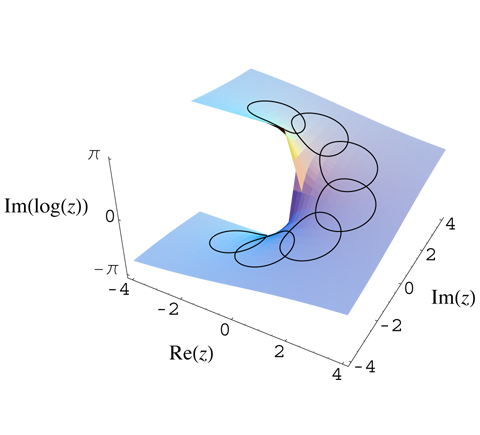
\includegraphics{images/Imaginary_log_analytic_continuation.png}
  In general, a Riemann surface is equivalent to the set of analytic
  continuations modulo the equivalence relation that two analytic
  continuations yield the same function at the endpoint.

  \section*{Laurent Series}
  \begin{defn}
    Let $f$ be an analytic function in annulus $\rho < |z-z_0| <
    \sigma$. Then, $f$ has \emph{Laurent decomposition} $f(z) = f_0(z)
    + f_1(z)$ where $f_0(z)$ is analytic on $|z-z_0| < \sigma$ and
    $f_1(z)$ is analytic on $|z-z_0| > \rho$ with normalization $f_1(\infty) = 0$.
  \end{defn}
  The Laurent decomposition is given by
  \begin{align*}
    f(z) & = \frac{1}{2 \pi i} \int_{\text{boundary}} f \\
    \ & = \frac{1}{2 \pi i} \int_{|z-z_0| = s} \frac{f(w)}{w-z} dw +
        \left( \frac{-1}{2 \pi i} \int_{|z-z_0| = r}
        \frac{f(w)}{w-z}dw \right), \ \rho < s < r < \sigma
  \end{align*}
  Where $f_0$ is the first summand and $f_1$ is the second
  summand. We note that $f$ always has a unique Laurent decomposition
  with the condition $f_1(\infty) = 0$. Now, we also note that $f_0$
  is analytic on a disk and $f_1$ is analytic on an exterior domain,
  so we get that
  \begin{align*}
    f = f_0+f_1 & = \sum_{k \geq 0} a_k(z-z_0)^k + \sum_{k \leq -1}
                  a_k(z-z_0)^k \\
    \ & = \sum_{k=-\infty}^\infty a_k(z-z_0)^k
  \end{align*}
  The astute reader will note that this series is indeed only defined
  on the annulus because the sum of these two power series $f_0$ and
  $f_1$ can only be defined on the intersection of their respective
  domains. We call this series the \emph{Laurent series}. The Laurent
  series equals $f$ on the annulus $\rho < |z-z_0| < \sigma$ and it
  converges uniformly on $r < |z-z_0| < s$ for $\rho < r < s <
  \sigma$. To compute these coefficients, we note that
  \begin{align*}
    \oint_{|z-z_0|} \frac{f(z)}{|z-z_0|^{n+1}} dz
    & = \sum_{k=-\infty}^\infty \int_{|z|=r} a_k \left(
      \frac{(z-z_0)^k}{(z-z_0)^{n+1}} dz \right) \\
    \ & = 2 \pi i a_n \\
    \implies a_n & = \frac{1}{2 \pi i} \int_{|z-z_0|}
                 \frac{f(z)}{(z-z_0)^{n+1}}dz
  \end{align*}
  Where the second to last equality comes from the fact that all those
  integrals are 0 unless $k=n$. Note that we also already had this
  result of power series on disks, $n \geq 0$.
  \begin{example}
    Consider $\frac{1}{z^2-z}$ on $0 < |z| < 1$. One way to find this
    Laurent series would be to note that \[
      \frac{1}{z^2-z} = \frac{-1}{z}\frac{1}{1-z} =
      \frac{-1}{z}(1+z+z^2+\cdots) = \frac{-1}{z}-1-z-z^2-\cdots
    \]
    Another way would be to use partial fractions to get that \[
      \frac{1}{z^2-z} = \frac{1}{z-1} - \frac{1}{z} =
      (-1-z-z^2-\cdots) - \frac{1}{z}.
    \]
    What about the function on $\frac{1}{z^2-z}$ on $1 < |z| (<
    \infty)$? We note that \[
      \frac{1}{z^2-z} = \frac{1}{z-1} - \frac{1}{z} =
      \frac{1}{z}\left(\frac{1}{1-\frac{1}{z}}\right) - \frac{1}{z} =
      \frac{1}{z}\left( 1 + \frac{1}{z} + \frac{1}{z^2} + \cdots \right) -
        \frac{1}{z} = \frac{1}{z^2} + \frac{1}{z^3} + \cdots
    \]
  \end{example}
  Thus, the entire domain can be covered by 2 Laurent series centered
  at 0 and $\infty$.  In general, it may require more series. For
  instance, consider the Laurent series valid on annuli centered at
  $z=i$. Since the function has problem points at $z=0,1$, it is clear
  that 3 different Laurent series will be needed. More generally for
  this function, the points 0,1, and $\Re z = \frac{1}{2}$ will only
  require 2 Laurent series, but centering at any other point will
  require 3. \\

  Just as a power series for $f$ at $z_0$ converges on the largest
  disk to which $f$ extends analytically, the Laurent series for $f$
  centered at $z_0$ converges on the largest annulus to which $f$
  extends analytically.

  \section{(10/20/2016) Lecture 16}
  \subsection*{Isolated Singularities}
  \begin{defn}
    $z_0$ is an isolated singularity of $f$ if $f$ is analytic on $0 <
    |z-z_0| < \epsilon$ for some $\epsilon$ but not at $z_0$.
  \end{defn}
  Given this situation, then $f$ has a Laurent series valid in a
  punctured disk at $z_0$, $\sum_{-\infty}^\infty a_k(z-z_0)^k$. We
  call the part with negative powers, $\sum_{k < 0} a_k(z-z_0)^k$ the
  \emph{principal part} or \emph{singular part}.

  \begin{itemize}
  \item If the principal part is empty, we say $z_0$ is removable.
  \item If the principal part has finitely many terms, we say $z_0$ is
    a pole of order $N$, where $-N$ is the least $k$ with $a_k \neq
    0$. e.g. $\frac{1}{z}+\frac{3}{z^2}$ has a pole of order 2 at 0.
  \item If the principal part has infinitely many terms, we say $z_0$
    is an essential singularity.
  \end{itemize}
  \begin{example}
    $\frac{\sin z}{z}$ has a removable singularity at 0. This is
    because its Laurent series is $\frac{z-\frac{z^3}{3!}+\cdots}{z} =
    1-\frac{z^2}{3!}+\frac{z^4}{5!}\cdots$. 
  \end{example}
  \begin{example}
    $\sin \frac{1}{z}$ has an essential singularity at 0. Examine its
    Laurent series: $\frac{1}{z}-\frac{1}{3!z^3}+\frac{1}{5!z^5}\cdots$.
  \end{example}
  \begin{prop}
    The following are equivalent for $f$ with isolated singularity at
    $z_0$.
    \begin{enumerate}[label=(\roman*)]
    \item $z_0$ is removable.
    \item $\lim_{z \to z_0} f(z)$ exists and is finite.
    \item $f$ is bounded in a deleted neighborhood of $z_0$.
    \end{enumerate}
  \end{prop}
  \begin{proof}
    (iii) implies (i) is Riemann's Theorem on Removable Singularities
    (see Gamelin p 172). We will prove this theorem. Assume $|f(z)|
    \leq A$ near $z_0$. We need $a_k = 0$ for $k < 0$. We note that \[
      a_k = \frac{1}{2 \pi i}\int_{|z-z_0|=r} \frac{f(z)}{(z-z_0)^{k+1}}dz
    \]
    where $r$ is small. Now, let us perform an ML-estimate on this
    integral. We get that $M = \frac{A}{r^{k+1}}$ and $L = 2\pi
    r$. Thus, \[
      |a_k| = \frac{1}{2\pi} \cdot \frac{A}{r^{k+1}} \cdot 2 \pi r = Mr^{-k}.
    \]
    Since $k < 0$ and this estimate is valid for small $r$, we get
    that $|a_k| = 0$.
  \end{proof}
  \begin{lem}
    Let $z_0$ be an isolated singularity of $f$. Then, the following
    are equivalent.
    \begin{enumerate}[label=(\roman*)]
    \item $z_0$ is a pole of order $N$.
    \item $\frac{1}{f}$ extends to $z_0$ with a zero of order $N$ at
      $z_0$.
    \item $f(z) = \frac{g(z)}{(z-z_0)^N}$ for $g$ analytic in
      neighborhood of $z_0$ where $g(z_0) \neq 0$. 
    \end{enumerate}
  \end{lem}
  When considering this lemma, one should be thinking of functions
  like $f(z) = \frac{1}{z^N}$.
  \begin{prop}
    Let $z_0$ be an isolated singularity of $f$. Then, $z_0$ is a pole
    if and only if $\lim_{z\to z_0} |f(z)| = \infty$.
  \end{prop}
  \begin{proof}
    The forward direction is obvious since it is part 3 of the
    previous lemma. For the backward direction, consider
    $\frac{1}{f}$. It is bounded near $z_0$, so $z_0$ is a removable
    singularity of $\frac{1}{f}$, and its extension has a zero of some
    order there. \[
      \frac{1}{f(z)} = g(z)(z-z_0)^N, g(z_0) \neq 0
    \]
    So, $f(z) = \frac{1}{g(z)}\frac{1}{(z-z_0)^N}$. Since
    $\frac{1}{g(z)}$ is analytic and not zero near $z_0$, this is a
    pole of order $N$.
  \end{proof}
  \begin{thm}[Casorati-Weierstrass]
    If $z_0$ is an essential singularity, then the image of any
    deleted neighborhood is dense in $\C$.
  \end{thm}
  \begin{example}
    Consider $e^{\frac{1}{z}}$ at $z=0$. 
  \end{example}
  \begin{proof}
    Supposed $z_0$ is an isolated singularity and there is
    $w,\delta,\epsilon$ so that $f(0 < |z-z_0| < \delta) \cap
    D_\epsilon(w) = \varnothing$. Then, $|f(z)-w| > \epsilon$ on
    $|z-z_0| < \delta$. This means that $\left| \frac{1}{f(z)-w}
    \right| < \frac{1}{\epsilon}$ on the deleted neighborhood. Now, by
    Riemann's theorem, $\frac{1}{f(z)-w}$ has a removable singularity
    at $z_0$. Therefore, $\frac{1}{f(z)-w} = g(z)(z-z_0)^N$ for some
    $N \geq 0$ and some analytic function $g(z)$ where $g(z_0) \neq
    0$. Then, we have that $f(z) = w + \frac{1}{g(z)}(z-z_0)^N$. So,
    if $N=0$, the singularity is removable. If $N > 0$, then the
    singularity is a pole of that order. In either case, the
    singularity is not essential, proving the contrapositive.
  \end{proof}
  \begin{defn}
    A function $f$ is \emph{meromorphic} on a domain $D$ if its only
    singularities are isolated points.
  \end{defn}
  Analytic is $f: D \to \C$ is also called holomorphic. Meromorphic is
  analogous on $f: D \to \C^*$.

  \section{(10/25/2016) Lecture 18}
  As a summary of our results from the previous lecture, we have the
  following table. \\
  \begin{tabular}{|c|c|}
    \hline
    Type & Behavior \\
    \hline
    Removable & Bounded; Equivalently, has a limit. \\
    Pole (with order) & $\lim_{z \to z_0} f(z) = \infty$ \\
    Essential & $f(D_\epsilon(z_0) \setminus \{z_0\})$ is dense in
                $\C$ for all $\epsilon$ \\
    \hline
  \end{tabular}
  Also, note that $f(z)$ has an isolated singularity at $\infty$ if
  and only if $f(\frac{1}{z})$ has an isolated singularity at 0. This
  is because if the Laurent series for $f(\frac{1}{z}) = \sum a_k
  z^k$, then $f(z) = \sum a_k z^{-k}$, which is the Laurent series for
  $f$ at $\infty$. Thus, the singular part at $\infty$ is $\sum_{k
    \leq 0} a_kz^{-k}$.
  \begin{example}
    If $f$ is a polynomial or any entire function, then $f$ is its own
    singular part at $\infty$. Eg $z^3+z+2$. 
  \end{example}
  Now, returning to the idea of meromorphic, we have the following
  examples.
  \begin{example}
    $\frac{1}{\sin z}$ is a meromorphic function on $\C$. It has
    infinitely many poles of order 1, but they are all
    isolated. However, this function is not meromorphic on
    $\C^*$. Poles in $\C$ accumulate at $\infty$. 
  \end{example}
  \begin{example}
    A polynomial is meromorphic on $\C^*$; it has one pole at
    $\infty$. Rational functions are also meromorphic on $\C^*$ by
    similar reasoning.
  \end{example}
  A fact worth noting. With $n = \max\{ \operatorname{deg} p(z),
  \operatorname{deg} q(z) \}$ and $p,q$ relatively prime, $z \mapsto
  \frac{p(z)}{q(z)}$ is $n$ to 1 from $\C^*$ to $\C^*$, including
  multiplicity.
  \begin{rmk}
    One can add, multiply, divide (but not by 0) meromorphic functions
    to get another meromorphic function. This follows from the fact
    that the poles all have finite order.
  \end{rmk}
  \begin{prop}
    All meromorphic functions on $\C^*$ are rational functions.
  \end{prop}
  \begin{proof}[Idea of proof]
    First, there are only finitely many poles, otherwise they ware not
    isolated because they would accumulate.

    Second, let $\{z_1, \ldots, z_j\}$ be the poles in $\C$. Let
    $p_j(z)$ be the principal part at $z_j$ and $p_\infty(z)$ be the
    principal part at $\infty$. Then $f - (p_\infty + \sum p_j)$ is an
    entire function that extends to be 0 at $\infty$.

    Third, it is bounded. So,

    fourth, by Liouville, it is zero. Thus, $p_\infty + \sum p_j$ is rational.
  \end{proof}
  Writing $f = p_\infty + \sum p_j$ is the partial fraction
  decomposition of $f$.
  \section{(10/27/2016) Lecture 19}
  So, we have now concluded that in complex analysis, a meromorphic
  function on $\C^*$ is the sum of the principal parts at (finitely
  many) poles.

  \subsection*{Residues}
  If $z_0$ is an isolated singularity of $f$, then $f(z) = \ldots
  a_{-1}(z-z_0)^{-1} + a_0 + a_1(z-z_0)+\ldots$. So, we have that \[
    \oint_{|z-z_0| = \epsilon} f(z)dz = \oint \sum_{-\infty}^{\infty}
    a_k(z-z_0)^k = \sum a_k
    \left(
      \oint (z-z_0)^kdz
    \right) = 2\pi i a_{-1}
  \]
  We say that $a_{-1}$ is the \emph{residue} of $f$ at $z_0$, written
  $\Res[f,z_0]$. Some examples:
  \begin{example}
    \begin{itemize}
    \item $\Res[\frac{10}{z},0] = 10$
    \item $\Res[\frac{1}{z^2},0] = 0$. Notice that the residue can be
      zero at a pole.
    \item $\Res[\frac{1}{z^2}e^{1/z},0] = 0$ because $e^{\frac{1}{z}}
      = 1 + \frac{1}{z} + \frac{1}{2!z^2} + \cdots$.
    \item $\Res[e^{\frac{1}{z^2}},0] = 0$ because $e^{\frac{1}{z^2}} =
      1+ \frac{1}{z^2} + \frac{1}{2! z^4} + \cdots$. 
    \end{itemize}
  \end{example}
  \begin{thm}[Residue theorem]
    Let $D$ be a bounded domain with piecewise smooth boundary. Let
    $f$ be analytic on $D \cup \partial D$ except for finitely many
    isolated singularities $z_1, \ldots, z_n$. Then, \[
      \oint_{\partial D} f(z)dz = 2 \pi i \sum_{j=1}^k \Res[f,z_j]
    \]
  \end{thm}
  The reason for this being true is to consider a path around the
  boundary (oriented correctly) and then also around each of the
  singularities (oriented clockwise). By the
  Cauchy Integral Theorem, this should be 0 and so, the integral
  around $\partial D$ is the same as the sum of the integrals around
  these singularities.

  Some rules for residues.
  \begin{enumerate}
  \item If $z_0$ is a simple pole of order $f$, then $\Res[f,z_0] =
    \lim_{z \to z_0} (z-z_0)f(z)$. Why? $f(z) = a_{-1}(z-z_0)^{-1} +
    a_0 + a_1(z-z_0) + \cdots$ so $(z-z_0) = a_{-1} + a_0(z-z_0) +
    a_1(z-z_0)^2 + \cdots$.
  \item If $z_0$ is a double pole of $f$, then $\Res[f,z_0] = \lim_{z
      \to z_0} \frac{d}{dz}((z-z_0)^2f(z))$ etc for higher order
    poles.
  \item If $f(z) = \frac{g(z)}{h(z)}$ analytic and $h(z)$ has a simple
    zero at $z_0$, then $\Res[f,z_0] = \frac{g(z_0)}{h'(z_0)}$.
  \end{enumerate}
  We can use these ideas to help us evaluate $\oint_{\partial D}
  f(z)dz$ or even to help evaluate real integrals.
  \begin{example}
    Consider $\int_{-\infty}^\infty \frac{x^2}{(x^2+1)^2}dx$. The
    solution is to consider $\int_{-\infty}^\infty
    \frac{z^2}{(z^2+1)^2}dz$ around a semicircle in the top half plane
    with radius $R$. We will call the circular part $C_R$. This way,
    we only care about the singularity at $i$. The integral around the
    whole boundary is $2 \pi i \sum \Res = 2 \pi i \Res[
    \frac{z^2}{(z^2+1)^2}, i]$. We note that $i$ is a double pole
    because we can factor $(z^2+1)^2 = (z+i)^2(z-i)^2$. So, we get
    that \[
      \Res[\frac{z^2}{(z^2+1)^2},i] = \frac{d}{dz}
    \left(
      \frac{z^2}{(z+i)^2}
    \right)|_{z=i} = \frac{-8i+4i}{16} = \frac{-i}{4}.
  \] Thus, the whole integral is $2 \pi i \frac{-i}{4} =
  \frac{\pi}{2}$
  Now, this gives us that \[
    \frac{\pi}{2} = \oint \frac{z^2}{(z^2+1)^2}dz = \int_{-R}^R
    \frac{x^2}{(x^2+1)^2}dx + \int_{C_R} \frac{z^2}{(z^2+1)^2}dz.
  \]
  We will attempt to bound the second integral by an ML-estimate. This
  gives us that $L = \pi R$ and $M = \frac{R^2}{(R^2-1)^2}$ so the
  integral is bounded by $\frac{\pi R^2}{(R^2-1)^2} \to 0$ as $R \to
  \infty$. Thus, \[
    \frac{\pi}{2} = \lim_{R \to \infty} \oint \frac{z^2}{(z^2+1)^2} dz =
    \int_{-\infty}^\infty \frac{x^2}{(x^2+1)^2}dx + 0
  \]
  \end{example}
  When doing such computations, make sure to do a reality check. When
  doing a real integral, the answer should be real. Ask, should it be
  positive? How big should it be?

  In general, what was necessary for our techniques to work on an
  integral of the form $\int_{-\infty}^\infty \frac{P(x)}{Q(x)}dx$? We
  needed $\operatorname{deg} Q \geq 2 + \operatorname{deg} P$ and
  $Q(x) \neq 0$ for $x \in \R$. The first condition was necessary so that our
  ML-estimate would tend to 0.
  \section{(11/1/2016) Lecture 20}
  Using residues, we can compute trig integrals. The idea is, for an
  integral of the form $\int_0^{2\pi} f(\theta) d\theta$ where $f$
  consists of trig functions, we can convert the integral to a complex
  integral using $z = e^{i \theta} \iff dz = ie^{i \theta}d\theta
  \implies d\theta = \frac{dz}{iz}$. Then, we rewrite the integral in
  terms of $z$ and integrate over $|z|=1$ and compute using residues.
  \begin{example}
    Consider $\int_0^{2\pi} \frac{\cos \theta}{2+\cos \theta}
    d\theta$. We note that $\cos \theta = \frac{e^{i \theta} + e^{-i
        \theta}}{2} = \frac{1}{2}(z+\frac{1}{z})$. Thus, our integral
    becomes \[\oint_{|z|=1}
    \frac{\frac{1}{2}(z+\frac{1}{z})}{z+\frac{1}{2}(z+\frac{1}{z})}
    \frac{dz}{iz}.\]
    We then compute the residues inside $|z|=1$ to get our final
    answer. Note that we would expect our answer to be between 0 and
    $2\pi$. A variation on this example would be an integral like
    $\int_{-\infty}^\infty \frac{\cos 2x}{(1+x^2)^2} dx$ which is
    solved by computing $\Re \int \frac{e^{iaz}}{(1+z^2)^2}dz$. 
  \end{example}

  \section{(11/3/2016) Lecture 21}
  We started this lecture discussing $d(\arg z)$ and how the value is
  dependent only on a path $\gamma$ and its winding number. We then
  asked what if $\gamma = f(\gamma')$ for some different path
  $\gamma' $. We then get $\int_{\gamma'} d(\log f(z)) =
  \int_{\gamma'} \frac{f'(z)}{f(z)}dz$ (we take $0 \not\in f(\gamma')
  = \gamma$). This is called the ``Logarithmic integral of $f$ on
  $\gamma'$.'' The takeaway is that \[
    \int_{\gamma'} \frac{f'(z)}{f(z)} dz = 2 \pi i (\text{winding
      number of }\gamma'\text{ around }0) = i(\text{change in argument
    on }\gamma').
  \]
  This leads us to a useful theorem.
  \begin{thm}
    Let $D$ be a domain with piecewise smooth boundary. Let $f$ be
    meromorphic on $D$ and extend continuoussly to the boundary
    $\partial D$. Then \[
      \oint_{\partial D} \frac{f'(z)}{f(z)} dz = 2\pi i (Z - P)
  \]
  Where $Z$ is the number of zeros in the domain and $P$ is the number
  of poles (counted with multiplicity). 
  \end{thm}
  \begin{proof}
    Let $z_1, \ldots, z_n$ be the zeros and poles of $f$ in $D$. Then,
    $f(z) = (z-z_0)^{N_k}g_k(z)$ where $g_k$ is analytic at $z_k$ and
    $g_k(z_k) \neq 0$ and $N_k$ is the order of the zero or minus the
    order of the pole. $\frac{f'(z)}{f(z)}$ is analytic off
    $\{z_k\}$. \[
      \frac{f'(z)}{f(z)} = \frac{N_k(z-z_k)^{N_k-1}g_k(z) +
        (z-z_k)^{N_k}g_k(z)}{(z-z_k)^{N_k}g_k(z)} = \frac{N_k}{z-z_k}
      + \frac{g_k'(z)}{g_k(z)}
    \]
    where we note that $\frac{g_k'(z)}{g_k(z)}$ is analytic at
    $z_k$. So, we get that $\Res(\frac{f'}{f},z_k) = N_k$ and
    $\frac{f'}{f}$ has simple pole at $z_k$. Thus, $\oint_{\partial D}
    \frac{f'(z)}{f(z)}dz = 2 \pi i \sum N_k$ by the Residue theorem,
    which is exactly $2 \pi i (Z-P)$. 
  \end{proof}
  \begin{example}
    What is the change in argument of $z^k$ on $|z|=1$
    counterclockwise? There are actually three different methods to
    compute this.
    \begin{enumerate}
    \item We note that $e^{i\theta}$ gets mapped to $e^{ik\theta}$ and
      so the change in argument is $2\pi k$.
    \item We could compute $\frac{1}{i} \oint_{|z|=1}
      \frac{kz^{k-1}}{z^k}dz = \frac{1}{i} \int \frac{k}{z}dz = 2\pi
      k$.
    \item $z^k$ has a zero of order $k$ at 0, so $2\pi i(Z-P) = 2\pi i
      k$ (where $Z$ is the number of zeros and $P$ is the number of
      poles). 
    \end{enumerate}
  \end{example}
  We are particularly interested in using this to count zeros of an
  analytic function in a region.
  \begin{example}
    Show $z^4+2z^3+3z^2+z+2$ has two zeros in the right hand
    plane. Our method is to compute $2\pi$ (number of zeros) $=
    \frac{1}{i} \int \frac{p'(z)}{p(z)}dz$, which is the change in
    argument on the boundary. \\

    So, let us consider a large semidisk in the right half plane with
    radius $R$. For large $R$, we need to count zeros inside the
    semidisk. This is exactly $\frac{1}{2\pi}$ change in argument of
    $p(\text{boundary})$ We need to check that this avoids 0. So, we
    note that \[
      p(iy) = (y^4-3y^2+2) + i(-2y^3+y) = (y^2-2)(y^2-1) -
      2y(y^2-\frac{1}{2})i.
    \]
    Now, we create a chart to look at the change across the zeros 
    \[    
    \begin{array}{ccccccccccccccc}
      &\sqrt{2}&&-1&&-\frac{1}{\sqrt{2}}&&0&&\frac{1}{\sqrt{2}}&&1&&\sqrt{2}&
      \\
      \Re p(iy) + &|& - &|& + &|& + &|& + &|& + &|& - &|& + \\
      \Im p(iy) + &|& + &|& + &|& - &|& + &|& - &|& - &|& -
    \end{array}
    \]
    Note, $p(iy)$ is not 0 for $y \in \R$, that is, real and imaginary
    parts have no common zeros on the imaginary axis. If we draw out
    these movements, we will get a path that does not wind around the
    origin. Then, we connect it by noting that the image of the
    half-circle is an arc with angle $4\pi$ since $p(z) \sim z^4$. Our
    final result is that the image is wrapped around twice. \\

    Next, we ask how many zeros are in the first quadrant? Since the
    polynomial has real coefficients, $z_0$ a root implies that
    $\overline{z_0}$ is also a root. Since $p(z)$ is positive for $z >
    0$ (by inspection), roots must be a conjugate pair, so one root in
    first quadrant and one in fourth quadrant. 
  \end{example}

  \subsection*{Integrands with branch points.}
  Integrands involving $\log x$ or $x^a$ have branch points and one
  way to deal with these is to integrate around a ``keyhole contour.'' \\
  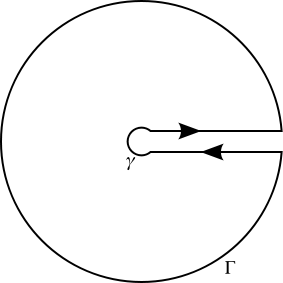
\includegraphics[scale=0.5]{images/keyhole_contour.png} \\
  \begin{example}
    Consider $\int_0^\infty \frac{x^{-a}}{1+x}dx, 0 < a < 1$. We will
    compute $\oint \frac{z^{-a}}{1+z}dz$ where the branch
    of $z^{-a}$ is $(re^{i\theta})^{-a} = r^{-a}e^{-ia\theta}$ for
    $\theta \in [0,2\pi)$. The final result was a homework question.
  \end{example}
\end{document}
